\section{Evaluation}
\label{sect:evaluation}
We have implemented and evaluated a prototype of our VC scheme on a Linux cluster of machines with
8-core 3.1Ghz AMD FX-8120 and 16 GB RAM. 
Our implementation is based on Alibaba cloud platform~\cite{Aliyun,WeiZhangIEEE}
and the underlying DFS uses  QFS with default replication degree 3 while the PDS replication degree is 6.
Our evaluation objective is to
study the benefit in fault tolerance and   deduplication efficiency of VC,  
and assess its backup throughput and  resource usage. 

We will compare VC with a VO approach  using stateless routing with binning (SRB) 
based on~\cite{Dong2011,extreme_binning09}.
SRB executes a distributed deduplication by routing a data chunk to one of cluster machines~\cite{Dong2011}
using  a min-hash function discussed in \cite{extreme_binning09}. Once a data chunk is routed to
a machine, the chunk is compared with the fingerprint index within this machine locally. 

\subsection{Settings}
We have performed a trace-driven study using a production dataset~\cite{WeiZhangIEEE} from 
Alibaba Aliyun's cloud platform with about 100 machines. 
Each machine hosts up to 25 VMs and each VM keeps 10 automatically-generated snapshots in the storage system while
a user may instruct extra snapshots to be saved.
The VMs of the sampled data set use popular operating systems such as 
Debian, Ubuntu, Redhat, CentOS, win2008 and win2003. 
%The backup of VM snapshots is required to complete within few  hours every night.
Based on our study of production  data,  each VM has about 40GB of storage  data  on average
including OS and user data disk.
%All data are divided into 2 MB fix-sized segments and 
The fingerprint for variable-sized chunks is computed using their SHA-1 hash~\cite{similar94,rabin81}. 
%Each segment is divided into 
%variable-sized content chunks with an average size of 4KB.
%Popularity of data blocks are collected through global counting and 
%and top popular ones ($\delta=2\%$)  are  kept in the PDS, as discussed in Section~\ref{sect:store}.

\subsection{Fault Isolation and Snapshot Availability}

 Table~\ref{tab:vm-availability} shows the availability of VM snapshots when 
there are up to 20 machine nodes failed in a 100-node cluster and  a 1000-node cluster. 
%Two VC curves use $V_c=1250$ and $V_c=2500$ representing the average number of VMs that share a PDS file system block. 
We have assumed a worst-case scenario that  a PDS block is shared by every VM. 
%($V_c=p*V$), which is to be expected when PDS
%blocks are sorted by hash, as their order is randomized.
%$V_c=2500$ represents  the absolute worst case for 2500 VMs. 
%The VO curve has  $V_o=6.3$ which is the average number of VMs that share a file system block in our smaller dataset.
%To get this number, we perform perfect deduplication over 105 VMs, append unique chunks to a DFS file and
%count the number of dependencies from a file system block to VM.
%In the scenario of having 2500 VMs, this number can only increase, thus this number represents the best
%case for VO approach. 
%Our results show that the VC approach even with $V_c=2500$ has a higher availability than VO.
%For example, with 10 machines failed, VO with 98.5\% availability would lose snapshots of 37 VMs 
%while VC with 99.9\% loses snapshots of 2.5 VMs.
%The key reason is that  $N_1 +N_2 < N_o$, caused by the fact that the VM-centric approach localizes deduplication
%and packs  data blocks for one VM as much as possible.  The extra replication
%for PDS blocks also significantly increases the snapshot availability even when
%a PDS file block is shared by every VM.
%=======
%Figure~\ref{tab:vm-availability} shows the availability of VM snapshots
%as storage nodes fail. 
%We assume a random distirbution of 64MB file system
%blocks (FSBs). where FSBs are not randomly distributed availability might
%be improved by limiting the number of storage nodes a particualr VM depends
%on but we take the conservative approach. We compare VO, the expected case for
%VC ($V_c=p*V/2$), and the worst case for VC ($V_c=p*V/2$). We set $V_o=6.3$
%based on measured values in our dataset.
%To obtain VO sharing of file blocks, we perform perfect deduplication over 105 VMs, 
%append unique chunks to a DFS file and
%count the number of dependencies from a file system block to VM.
%In the case of having 2500 or even 25000 VMs, this number can only increase, thus this number represents the best
%case for VO approach. 
Our results show that even the worst case,  VC  still has a significantly  higher availability than VO as the number of
failed machines increases.
%Our VM-centric approach shows significant improvements
%in VM availability.
For example, with 5/100 machines failed and 25 VMs per machine, VO with 93.256\% availability would lose data in 169 VMs 
while VC with 97.763\% loses data for 56 VMs.
The key reason is that for most data in VC, only a single
VM can be affected by the loss of a single FSB. Since most FSBs contain chunks for a single VM, VMs can depend on a smaller number of FSBs.
% because our VM-centric approach
%localizes deduplication.  

Although the loss of a PDS block affects many VMs,
by increasing replication for those blocks we minimize the effect on VM snapshot availability.
%By having extra replicas for the PDS data, we reduce the failure rate of PDS
%FSBs enough that the failure rate for the VM approaches the failure rate of the
%Non-PDS blocks. This minimizes the drop in availability between the expected
%and worst case for VC.
%
%One of the advantages of VC is that there is a division between
%popular and non-popular data to facilitate improved reliability. 
Figure~\ref{fig:pds-replication} shows
the impact of increasing PDS data replication. 
While the impact on storage cost is small, 
a replication degree of 6  has a significant improvement over 4, but the availability is about
the same for $r_c=6$ and $r_c=9$ (beyond $r_c=6$ improvements are minimal).
 
%This is because, as described before, the availability of the VM approaches the
%availiability of the Non-PDS data as the failure rate of PDS data gets very small.

\comments{
\begin{figure}[ht]
    \centering
    \begin{subfigure}%{.5\textwidth}
      \centering
      %\includegraphics[scale=.45,natwidth=511,natheight=276]{vo_links}
            \begin{tikzpicture}
                    \begin{axis}[
                    tick label style={font=\scriptsize},
                    tick style=thin,
                    width=0.5\linewidth,
                    title={\small $p=100$},
                    cycle list={
                        {blue,thin,solid,mark=none},
                        {red,thin,densely dashed,mark=none},
                        {red,thin,densely dotted,mark=none}
                    },
                    xlabel={\tiny Failed nodes},
                    ylabel={\tiny Snapshot Availability (\%)},
                    %extra y ticks={99.9}, %if important numbers are missing
                    mark options=solid,
                    legend columns=-1,
                    legend style={
                        font=\small\sffamily,
                        cells={anchor=west}, %legend entry alignment
                        legend pos=south west %legend position
                    },
                    legend to name=legend:vm-availability,
                    %reverse legend,
                    ]
                    \addplot table[x=NodesFailed,y=VO]{figures/node_failures_100.txt};
                    \addlegendentry{VO}
                    \addplot table[x=NodesFailed,y=VC3]{figures/node_failures_100.txt};
                    \addlegendentry{VC}
                    %\addplot table[x=NodesFailed,y=VCOpt1]{figures/node_failures_100.txt};
                    %\addlegendentry{VC (CDS ordering)}
                    \end{axis}
            \end{tikzpicture}
      %\caption{100 machine cluster.}
      \label{fig:vm-availability-100}
    \end{subfigure}%
    \begin{subfigure}%{.5\textwidth}
  \centering
  %\includegraphics[scale=.45,natwidth=511,natheight=276]{vo_links}
	\begin{tikzpicture}
            %the expressions in this plot are simply to trick pgfplots into not expanding the y range, and don't actually change the data
            % expression used: (99.999+((y-99.999)*1000)/1000)
            \pgfplotsset{/pgf/number format/.cd,
                fixed,precision=4}
		\begin{axis}[
                    width=0.5\linewidth,
                    tick label style={font=\scriptsize},
                    tick style=thin,
		title={\small $p=1000$},
                %ymin=099.9991,
                %ymax=100.0002,
                %ytick=data,
                %yticklabels from table={figures/vm_availability_1000.txt}{[index]1},
                yticklabel={%this is a hack to get around the small yrange
                    \pgfmathfloatparse{99.999+\tick/1000}
                    \pgfmathprintnumber{\pgfmathresult}
                },
                cycle list={
                    {blue,thin,solid,mark=none},
                    {red,thin,densely dashed,mark=none},
                    {red,thin,densely dotted,mark=none}
                },
		xlabel={\tiny Failed nodes},
		ylabel={\tiny Snapshot Availability (\%)},
		%extra y ticks={99.99}, %if important numbers are missing
                mark options=solid,
                legend style={
                    cells={anchor=west}, %legend entry alignment
                    legend pos=south west %legend position
                },
                %reverse legend,
		]
                %\addplot table[x=NodesFailed,y=VO1]{figures/vm_availability_1000.txt};
                \addplot table[x=NodesFailed,y expr=(\thisrow{VO}-99.999)*1000]{figures/node_failures_1000.txt};
                %\addlegendentry{$VO\,6.3$ (optimistic)}
                %\addplot table[x=NodesFailed,y=VC1]{figures/vm_availability_1000.txt};
                \addplot table[x=NodesFailed,y expr=(\thisrow{VC3}-99.999)*1000]{figures/node_failures_1000.txt};
                %\addlegendentry{$VC\,1250$ (estimated)}
                %\addplot table[x=NodesFailed,y=VC2]{figures/vm_availability_1000.txt};
                \addplot table[x=NodesFailed,y expr=(\thisrow{VCWC1}-99.999)*1000]{figures/node_failures_1000.txt};
                %\addlegendentry{$VC\,2500000$ (worst-case)}
                %\addplot table[x=NodesFailed,y=VO2]{figures/vm_availability.txt};
                %\addlegendentry{$VO\,20$ (optimistic)}
		\end{axis}
	\end{tikzpicture}
        %\caption{1000 machine cluster.}
  \label{fig:vm-availability-1000}
\end{subfigure}
    \pgfplotslegendfromname{legend:vm-availability}
      \caption{Availability of VM snapshots for VO and VC when failed machines vary
from 1 to 40.  Non-PDS replication is fixed
at 3 and PDS replication is 6 \emph{THIS PLOT IS BEING REPLACED BY A TABLE} 
      }
      \label{fig:vm-availability}
   
 
\end{figure}
}
\begin{table}
  \centering
    \footnotesize
    \tabcolsep=0.11cm
    \pgfplotstabletypeset[
        columns={NodesFailed,VO100,VC100,VO1000,VC1000},
        columns/NodesFailed/.style={
            column name={\multirow{3}{*}{Failures ($d$)}}
        },
        columns/VO100/.style={
            column name={
                \multicolumn{4}{c|}{VM Snapshot Availability(\%)}\\&
                \multicolumn{2}{c|}{$p=100$}&\multicolumn{2}{c|}{$p=1000$}\\&
            VO},
            fixed, precision=6
        },
        columns/VC100/.style={
            column name={VC},
            fixed, precision=6},
        columns/VO1000/.style={
            column name={VO},
            fixed, precision=6},
        columns/VC1000/.style={
            column name={VC},
            fixed, precision=6},
        every head row/.style={
            before row={\hline},
            after row={\hline},
        },
        every last row/.style={after row=\hline},
        column type/.add={}{|},
        every first column/.style={column type/.add={|}{}},
        %the below rows can be used to extract rows 3,5,10,20 from rows 0-40
        %skip rows between index={0}{3},
        %skip rows between index={4}{5},
        %skip rows between index={6}{10},
        %skip rows between index={11}{20},
        %skip rows between index={21}{41}
    ]{figures/availability_table.txt}
    \caption{Availability of VM snapshots for VO and VC.}
    \label{tab:vm-availability}
\end{table}


\begin{figure}[htbp]
  \centering
	\begin{tikzpicture}
		\begin{axis}[
                        width=\linewidth,
                        height=0.6\linewidth,
		%title={PDS Replication affect on availability},
		xlabel={Failed storage nodes},
		ylabel={VM Snapshot Availability (\%)},
                xmin=0,
                xmax=20,
		%extra y ticks={99.9}, %if important numbers are missing
                mark options=solid,
                legend style={
                    cells={anchor=west}, %legend entry alignment
                    legend pos=south west %legend position
                },
                reverse legend,
		]
                \addplot+[dashed] table[x=NodesFailed,y=VO]{figures/node_failures_100.txt};
                \addplot table[x=NodesFailed,y=VC1]{figures/node_failures_100.txt};
                \addplot table[x=NodesFailed,y=VC2]{figures/node_failures_100.txt};
                \addplot table[x=NodesFailed,y=VC3]{figures/node_failures_100.txt};
                \addplot table[x=NodesFailed,y=VC4]{figures/node_failures_100.txt};
                \legend{
                    VO,
                    $r_c=4$,
                    $r_c=5$,
                    $r_c=6$,
                    $r_c=9$
                }
		\end{axis}
	\end{tikzpicture}
  \caption{Availability of VM snapshots in VC with different PDS replication degrees}
  \label{fig:pds-replication}
\end{figure}

\subsection{Deduplication Efficiency}
\label{sect:evaldedup}

%this version combines the old and the minhash alg. to compare against srb
\begin{figure}[ht]
  \centering
    \begin{tikzpicture}
            \begin{axis}[
            %title={Ex-Binning Efficiency},
            width=\linewidth,
            height=0.75\linewidth,
            cycle list={%
                {blue,solid,mark=square*},
                {blue,solid,mark=triangle*,mark size=1.5},
                {blue,solid,mark=diamond*,mark size=1.5},
                %{blue,solid,mark=pentagon*,mark size=1.4},
                {red,draw=red,dotted,mark=square},
                %{red,densely dotted,mark=triangle,mark size=1.5},
                %{red,densely dotted,mark=diamond,mark size=1.5},
                {brown,dashed,mark=*},
                %{red,densely dotted,mark=o},
                %{red,densely dotted,mark=pentagon,mark size=1.4},
            },
            mark repeat={10},
            xlabel={Number of VMs added},
            ylabel={Dedup. Efficiency (\%)},
            xmin=0,
            ymin=85,
            ymax=100,
            %extra y ticks={4.5,5.5,6.5} %to add extra ticks
            mark options=solid,
            legend pos=south west,
            legend columns=2,
            legend style={
                font={\tiny\sffamily},
                nodes={right}
                %at={(0.5,-0.2)},
                %anchor=north
            },
            ]
            \addplot table[x=VMs,y=MHcds4] {figures/exbin_efficiency_comparison2.txt};
            \addplot table[x=VMs,y=MHcds2] {figures/exbin_efficiency_comparison2.txt};
            %\addplot table[x=VMs,y=MHcds1] {figures/exbin_efficiency_comparison2.txt};
            \addplot table[x=VMs,y=MHNocds] {figures/exbin_efficiency_comparison2.txt};
            %\addplot table[x=VMs,y=cds4] {figures/exbin_efficiency_comparison2.txt};
            \addplot table[x=VMs,y=cds2] {figures/exbin_efficiency_comparison2.txt};
            %\addplot table[x=VMs,y=cds1] {figures/exbin_efficiency_comparison2.txt};
            \addplot table[x=VMs,y=exbin] {figures/exbin_efficiency_comparison2.txt};
            \legend{VC( $\sigma=4\%$),
                VC($\sigma=2\%$),
                %VC MH($\sigma=1\%$),
                VC(No PDS),
                %VC($\sigma=4\%$),
                VC($\sigma=2\%$\, No similarity guidance),
                %VC($\sigma=1\%$),
                SRB
            };
            \end{axis}
    \end{tikzpicture}
    \caption{Deduplication efficiency of VC and SRB.}
  \label{fig:exbin-efficiency-graph2}
\end{figure}

Figure~\ref{fig:exbin-efficiency-graph2} shows the deduplication efficiency for SRB and VC,
% <<<<<<< HEAD
% Our deduplication efficiency is defined as the percent of duplicate chunks
% which are detected and deduplicated, so only global perfect deduplication can have 100\% efficiency.
% The figure also compares several PDS sizes chosen for VC. ``$\sigma=2\%$'' 
% is defined in Table~\ref{tab:symbol}. 
% =======
namely the percent of duplicate chunks
which are detected and removed.
% so only global perfect deduplication can have 100\% efficiency.
% We also compare several PDS sizes chosen for VC.
%(see Table~\ref{tab:symbol} for definition of ``$\sigma=2\%$'')
%we allocate the space of distributed shared memory  to accommodate 2\%
%of data chunks shared among VMs, as defined in 
With $\sigma=2\%$, memory usage for PDS index lookup per machine is about 100MB per machine
and  the deduplication efficiency can reach over 96.33\%.
When $\sigma=4\%$, the deduplication efficiency can reach 96.9\% while space consumption increases to 200MB per machine. 
%and  the deduplication efficiency can reach 96.489\%.
%When $\sigma=4\%$, the deduplication efficiency can reach 97.027\% while space consumption increases to 200MB per machine. 
The loss of efficiency in VC is caused by the restriction of the physical memory available
in the cluster for fast in-memory PDS index lookup. 
%In the extreme case if we put all the fingerprint into PDS 
%index ($\sigma=100\%$) then VC will have 100\% efficiency.
SRB can deliver up to 97.79\% deduplication efficiency which is slightly better than VC.
Thus this represents a tradeoff that VC provides better fault tolerance and fast approximate deletion
with competitive deduplication efficiency.

% SRB can deliver up to 97.935\% deduplication efficiency which is slightly better than VC.
% Thus this represents a tradeoff: VC provides better fault tolerance and fast
% approximate deletion with competitive (but slightly lower) deduplication
% efficiency.
% >>>>>>> 4dcd68612b052c0f890ed30361a9ed03771b5df1
%its loss of efficiency is caused by the routing of data chunks which restricts the search scope
%of duplicate detection.
%SRB provides slightly better deduplication efficiency than our VC approach, which we accept
%because we are rewarded by architecture-wise benefits such as fault-tolerance and fast 
%Though not our primary goal, this result does show that VC can remove competitive amount of duplicates.

Figure~\ref{fig:exbin-efficiency-graph2} also shows the curve  of VC without local similarity search.
There is a big efficiency drop in this curve when the number of VMs is about 30.
The reason is that  
%Without this (i.e. when we only 
when a data  segment is moved to another location on disk, for example when a file is rewritten
rather than modified in place,  
a dirty-bit or offset based detection would not be able to detect such a movement and 
similarity search becomes especially important.  We have found that in
approximately 1/3 of the VMs in our dataset this movement happens frequently.
In general, adding local similarity-guided search increases deduplication efficiency from 93\% to over 96\%.
That is one significant improvement compared to the work in ~\cite{WeiZhangIEEE}
which uses the parent segment at the same offset to detect duplicates instead of similarity-guided search.
% In general, our experiments show that
% dirty-bit detection at the segment level can reduce the data size to about 24.14\% of original data, 
% which leads about a 75.86\% reduction.
% Similarity-guided local search can further reduce the data size
% to about 12.05\% of original size, namely it delivers an additional 12.09\% reduction.
% The PDS-based global duplicate detection with $\sigma=2\% $
% can reduce the size further to 8.6\% of original size, namely it 
% delivers an additional 3.45\% reduction.

In general, our experiments show that
dirty-bit detection at the segment level can reduce the data size to about 24.14\% of original data, 
which leads to about a 75.86\% reduction.
Similarity-guided local search can further reduce the data size
to about 12.05\% of original, namely it delivers a 50.08\% reduction to the dirty segments.
The popularity-guided global deduplication with $\sigma=2\% $
can reduce the data further to 8.6\% of its original size, so
it provides additional 28.63\% reduction to the remaining data.

%Figure~\ref{fig:exbin-efficiency-graph2} also shows the benefits of our minhash
%similar segment search in the parent snapshot. 

\subsection{Resource Usage and Processing Time}

\comments{
\begin{table}
    \begin{tabular}{|c|c|}
    \hline
    PDS replication degree & Disk usage per machine  \\ \hline
    3                      & 3065GB             \\ \hline
    4                      & 3072GB             \\ \hline
    5                      & 3079GB             \\ \hline
    6                      & 3086GB             \\ \hline
    7                      & 3093GB             \\ \hline
    \end{tabular}
\caption{Storage space cost per machine for DFS under different PDS replication degree}
\label{tab:replication_cost}
\end{table}
}

{\bf Storage cost of replication.} 
%Table ~\ref{tab:replication_cost} shows the total storage space required by 
%VC as the PDS replication degree changes while non-PDS replication degree is fixed as 3. 
When the replication degree of both PDS and non-PDS data is 3, 
the total storage  for all VM snapshots in each physical machine takes about 3.065TB on average before compression
and 0.75TB after compression.  Allocating  one extra  copy for PDS data only adds  7GB in total per machine.
Thus PDS replication degree 6 only increases the total space by 0.685\% while PDS replication degree 9 adds 1.37\% 
space overhead, which is still small.
%The increase in storage cost is minimal because the PDS makes up a 
%small percent of the total storage space, while increasing replication degree has a  more significant benefit for
%availability as shown in Figure~\ref{fig:pds-replication}.

\begin{table}
    \begin{tabular}{|c|c|c|c|c|c|}
    \hline
    Tasks & CPU & Mem &Read &  Write  & Time  \\ 
    & & (MB)          &(MB/s) &  (MB/s) & (hrs) \\ \hline
%    1     & 19\% & 118.1 & 50MB/s 8.37 & 1.314\\ \hline
    1     & 19\% & 118 & 50 & 16.4 & 1.31\\ \hline
%    2     & 35\% & 131.8 & 9.0 & 1.226\\ \hline
    2     & 35\% & 132 &50  & 17.6 & 1.23\\ \hline
    %4     & 63\% & 154.1 & 9.3 & 1.179\\ \hline
    4     & 63\% & 154&50   & 18.3 & 1.18\\ \hline
    6     & 77\% & 171.9 & 50 &  18.8 & 1.162\\ \hline
%    8     & 82\% & 90.5 & 89.2 & \\ \hline
%    10                      & 85\% & 97.2   & 90.4 \\ \hline
%    12                      & 91\% & 95.6    & 91.5 \\ \hline
    \end{tabular}
\caption{Resource usage of concurrent backup tasks at each machine}
\label{tab:resource_usage}
\end{table}

{\bf Memory and disk bandwidth usage with multi-VM processing}. 
We have further studied the memory and disk bandwidth usage 
when running concurrent VM snapshot backup on each machine with $\sigma=2\%$. 
Table ~\ref{tab:resource_usage} gives the resource usage  when
running 1 or multiple  VM backup tasks at the same time on each physical machine. 
``CPU'' column is the percentage of a single core used. 
``Mem'' column includes 100MB memory usage for PDS index and other space cost for executing deduplication tasks such as 
receipt metadata and cache. 
``Read'' column is controlled as 50MB/s bandwidth usage with I/O throttling so that other cloud services are not impacted too much.
The peak read performance is about 300MB and we only use 16.7\% with this collocation consideration.
``Write'' column is the I/O write usage of QFS and notice that each QFS write leads writes in multiple machines due to
data replication.     50MB dirty segment read speed triggers about 16.4MB/second disk write for non duplicates with one backup task.
% [ NOT REASONABLE: Notice that memory and CPU used by PDS index and QFS are not included since they belong to 
% the cloud infrastructure services and are shared among many applications.]
%We see our hybrid deduplication scheme only occupies a small amount of system resources. 
%The  local deduplication only needs to keep the parent snapshot recipe and a few similar segment recipes in 
%memory during duplicate detection.

Table ~\ref{tab:resource_usage} shows that  a single backup task per node can complete the backup of the entire
VM cluster in about 1.31 hours. Since there are about 25 VMs per machine, we could execute
more tasks in parallel at each machine. But adding more backup concurrency does not shorten the overall time
significantly because of the controlled  disk read time.
%,  we can still process raw data at near 175 MB/s. If we consider the extreme case in which each machine has 25 VMs
%at 40GB size, our snapshot system can finish backing up all the VMs (1TB total) in 1.58 hours.

{\bf Processing Time breakdown}.
Figure~\ref{fig:vc_srb_combined} shows
the  average  processing  time of  a VM segment under VC and SRB. 
VC uses $\sigma=2\%$ and $4\%$.
It has a breakdown of processing time.
``Snapshot read/write'' includes snapshot reading and writing from disk, and 
updating of the metadata.
`` Network transfer" includes the cost of transferring raw and meta data from one machine to another during 
snapshot read and write.
``Index access/comparison'' includes the disk, network and CPU time during fingerprint comparison.
This includes PDS data lookup for VC and index lookup from disk in VO after Bloom filter lookup.
For VC, the change of $\sigma$ does not significantly affect the overall backup speed as
PDS lookup takes only a small amount of time.
While the amount raw data transferred in network is about the same for VC and SRB, 
SRB spends slightly more time for snapshot read/write because each snapshot  backup, more smaller bins are involved
 in  SRB while VC only involves fewer containers with a bigger size. Thus I/O aggregation is more effective in VC.
SRB has a higher cost for index access and fingerprint comparison because most of  chunk fingerprints are routed
to remote machines for comparison while   VC handles most of chunk fingerprints locally. 

%on the index holding machine to access its index (often on the disk, supported by a Bloom filter) 
%and perform comparison.
%VC is faster in this regard because it conducts in-memory local search first and then
%accesses  the PDS on distributed shared memory, so most chunks can be dealt with locally.  
%SRB spends  slighter more time in  reading data and updates because it also updates the on-disk
%local meta data index in addition to partition indices.
%As a result Overall,  VC is faster than SRB, though data reading dominates the processing time for both algorithms.
%Figure~\ref{fig:vc_srb_combined} also reports the average backup time for a VM in VC when
%varying the PDS size.  It lists the time distribution for data reading,
%similarity-guided local search, global PDS lookup, and non-duplicate data writing. 
%While data reading dominates the backup process, PDS lookup spends about a similar amount
%of time as local search.

\begin{figure}[htbp]
  \centering
  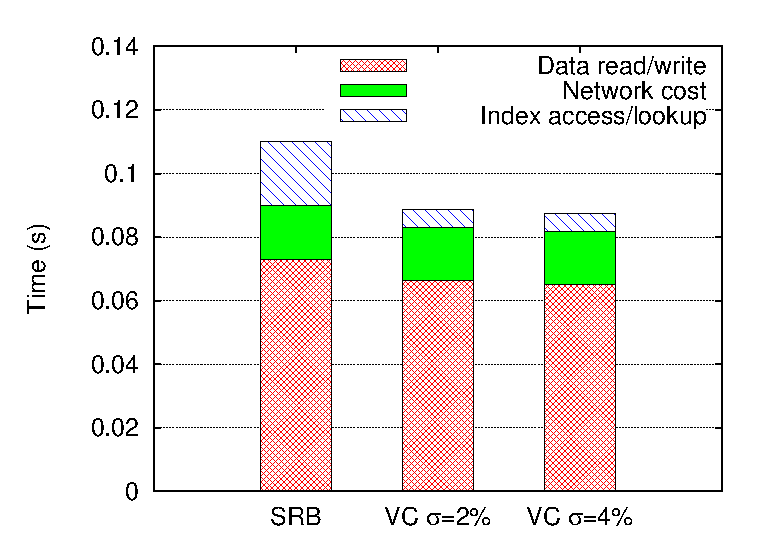
\epsfig{file=figures/vc_srb_combined, width=3in}
  \caption{Average time to backup a dirty VM segment under SRB and VC}
  \label{fig:vc_srb_combined}
\end{figure}

% \begin{figure}[htbp]
%   \centering
%   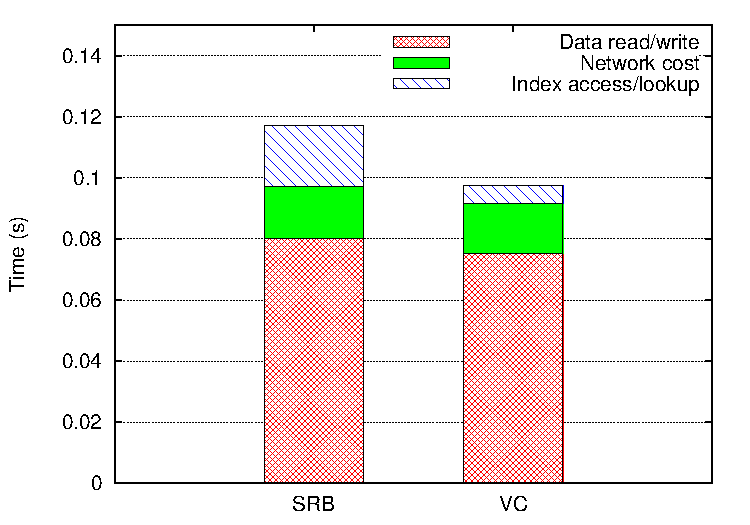
\epsfig{file=figures/srb_vs_vc, width=3in}
%   \caption{Time to backup a dirty VM segment under SRB and VC}
%   \label{fig:srb_vs_vc}
% \end{figure}


% \begin{figure}
%     \centering
%     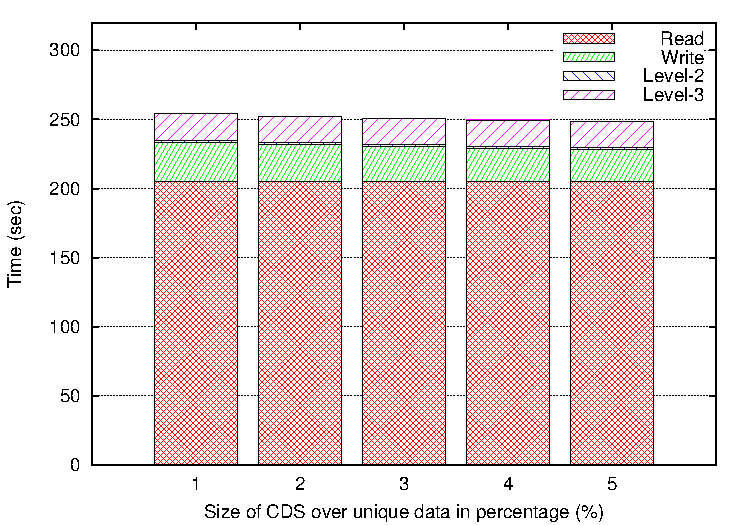
\includegraphics[width=3in]{figures/single_backup_time}
%     \caption{Average time to backup a VM in VC with varying PDS sizes}
%     \label{fig:single_vm_backup}
% \end{figure}


% \begin{table*}[t]
%     \centering
%     \begin{tabular}{c|ccc|ccc}
%     Num. of concurrent      & \multicolumn{3}{c|}{Throughput without}    & \multicolumn{3}{c}{Throughput with} \\
%     backup tasks            & \multicolumn{3}{c|}{I/O throttling (MB/s)} & \multicolumn{3}{c}{I/O throttling (MB/s)} \\ \cline{2-7}
%     per node                & Raw                                        & Snapshot Store & QFS  & Raw                                    & Snapshot Store & QFS  \\ \hline
%     1                       & 1369.6                                     & 148.0          & 18.0 & 171.3                                  & 18.5           & 2.26 \\
%     2                       & 2408.5                                     & 260.2          & 31.7 & 201.3                                  & 21.8           & 2.66 \\
%     4                       & 4101.8                                     & 443.3          & 54.1 & 217.8                                  & 23.5           & 2.87 \\
%     6                       & 5456.5                                     & 589.7          & 72.0 & 224.1                                  & 24.2           & 2.96 \\
%     \end{tabular}
% \caption{Throughput of software layers under different concurrency}
% \label{tab:throughput}
% \end{table*}
\begin{table}[htbp]
\begin{small}
    \centering
    \begin{tabular}{|c|ccc|}
\hline
    Concurrent      & \multicolumn{3}{c|}{Throughput without}    \\
    backup tasks            & \multicolumn{3}{c|}{I/O throttling (MB/s)} \\ \cline{2-4}
    per machine                & Backup                                     & Snapshot Store & QFS  \\ 
    		&                                      & (write) & (write)  \\ \hline
    1                       & 1369.6                                     & 148.0          & 35.3 \\
    2                       & 2408.5                                     & 260.2          & 61.7 \\
    4                       & 4101.8                                     & 443.3          & 103.1 \\
    6                       & 5456.5                                     & 589.7          & 143.8 \\ \hline
    \end{tabular}
\end{small}
\caption{Throughput of software layers per machine under different concurrency}
\label{tab:throughput}
\end{table}

{\bf Throughput of software layers.}
Table~\ref{tab:throughput} shows the  average throughput of software layer
when when I/O throttling is not applied to control the usage.
%machine when all machine nodes execute one or multiple MV backup tasks.
``Backup'' column is the throughput  of the backup service  per machine.
``Snapshot store" is the  write throughput of the snapshot store layer. The gap between this
column and  ``Backup" column is caused by significant data reduction by dirty bit and duplicate
detection. Only non-duplicate chunks trigger a snapshot store write.
``QFS'' column is the write request traffic to the underlying file system after compression.
For example, with 148MB/second write traffic to the snapshot store, QFS write traffic is about 35.3MB/second
after compression.  The underlying disk storage traffic will be three times greater with replication.
The result shows that the backup service can deliver up to 5.46GB/second without I/O restriction
per machine with 6 concurrent backup tasks. With a higher disk storage bandwidth available, the above backup
 throughput would be higher. 
%With 50MB/second controlled I/O bandwidth, each machine can deliver 171MB/second with 1 backup task and can complete the backup of 25 VMs per machine in less than 1.31 hours.
 
%To begin, on each node we write snapshots for 4 VMs concurrently, and gradually 
%increase number of VMs to 12 to saturate our system capability. 
%We observed 
%the per-node throughput peaked at 2700 MB/s when writing 10 VM snapshots in parallel, 
%which is far beyond our QFS file system capability. The reason behind it is our efficient
%deduplication architecture and compression which greatly reduce the amount of data that needs to be written to
%the file system. The main bottleneck here is that our QFS installation only
%manages one disk per node, which prevents it from fully utilizing the
%benefits of parallel disk access. We expect our architecture can
%perform even better in production clusters, which often have ten or more disks on each node.


% \begin{figure}
%     \centering
%     \subfigure[Backup throughput per node under controlled I/O bandwidth usage]
%     {
%         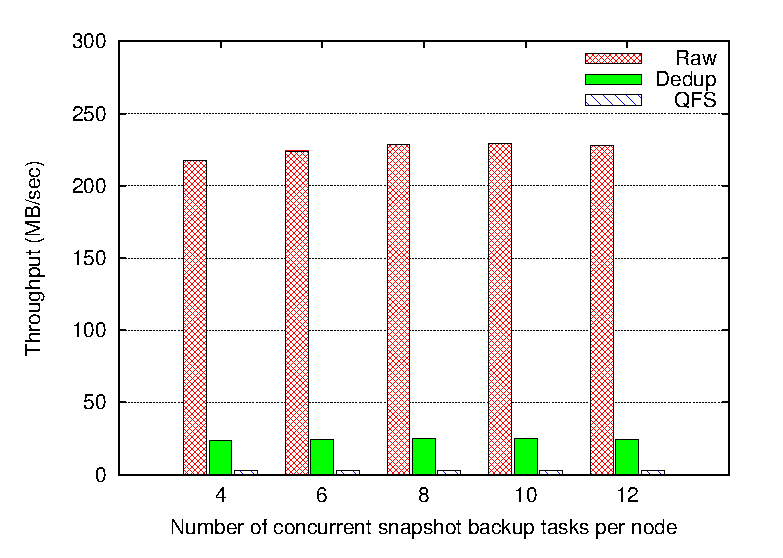
\includegraphics[width=3in]{figures/parallel_backup_with_read}
%         \label{fig:withread}
%     }
%     \\
%     \subfigure[Deduplication and storage system performance]
%     {
%         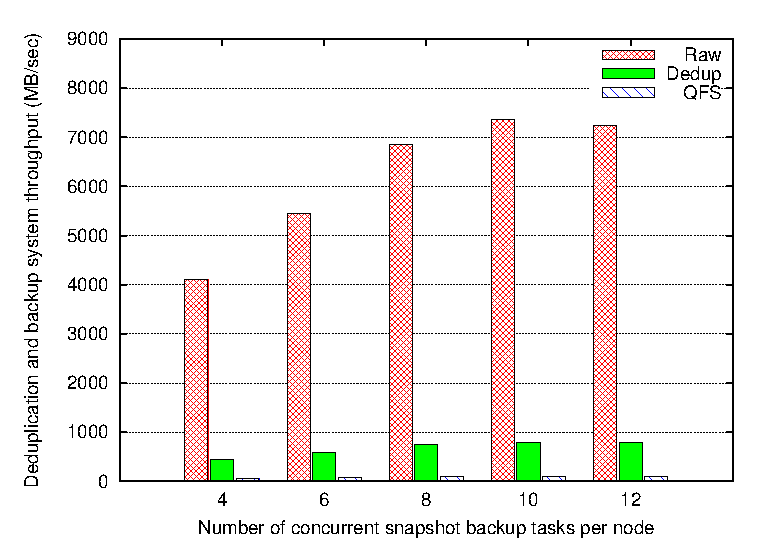
\includegraphics[width=3in]{figures/parallel_backup_no_read}
%         \label{fig:noread}
%     }
%     \caption{Throughput per-node with concurrent snapshot backup tasks}
%     \label{fig:parallel_backup}
% \end{figure}

 \subsection{Effectiveness of Approximate Deletion}

 \begin{figure}
     \centering
     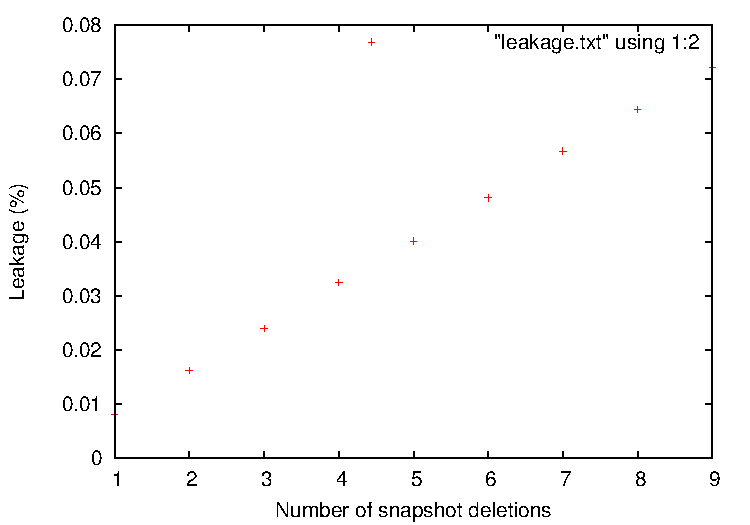
\includegraphics[width=3in]{figures/leakage}
     \caption{Accumulated storage leakage by approximate snapshot deletions ($\Delta u/u=0.025$)}
     \label{fig:leakage}
 \end{figure}

Figure~\ref{fig:leakage} shows the average accumulated storage leakage in terms of percentage of
storage space per VM caused  by approximate deletions.
The top dashed line is the predicted leakage using Formula~\ref{eq:leakrepair} from Section~\ref{sect:delete}
given $\Delta u/u=0.025$,
while the solid line represents the actual leakage measured during the experiment. 
The Bloom filter setting is based on $\Delta u/u=0.025$.
After 9 snapshot deletions, the actual leakage ratio reaches 0.0015 and this means that
there is only 1.8MB space leaked for every 1GB of stored data.
The actual leakage can reach  4.1\% after  245 deletions.
% We also measure the storage leakage under $\Delta u/u=0.05$ and $0.10$ settings for summary vectors.
% As this value increases, larger summary vectors are generated thus results in a decrease on the
% false-positive ratio, therefore less amount of unused chunks are misjudged. 
